% The boundary d_2 of a 2-cell e^2 is a sum of the 1-cells on its rim.
% Source: book/tex/homology/cellular.tex (§ The cellular boundary formula).
\documentclass[border=2mm]{standalone}
\usepackage{tikz}
\usepackage{amssymb}
\usepackage{amsmath}
\usetikzlibrary{arrows.meta,decorations.markings}
\tikzset{midarrow/.style={postaction={decorate},decoration={
  markings,mark=at position 0.55 with {\arrow{Latex[length=2mm]}}}}}
\begin{document}
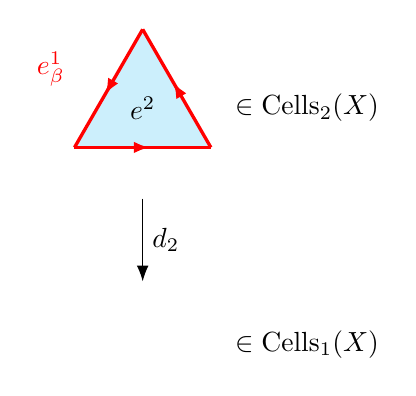
\begin{tikzpicture}[scale=1]
  % 2-cell e^2 (triangle), centred near (0,3).
  \fill[cyan!20] (90:1) -- (210:1) -- (-30:1) -- cycle;
  \draw[red, line width=1.2pt, midarrow] (-30:1) -- (90:1);
  \draw[red, line width=1.2pt, midarrow] (90:1) -- (210:1);
  \draw[red, line width=1.2pt, midarrow] (210:1) -- (-30:1);
  \node at (0,0) {$e^2$};
  \node[red, left] at (150:1) {$e^1_\beta$};
  \node[right] at (1.05,0) {$\in \operatorname{Cells}_2(X)$};
  % Arrow d_2 downward.
  \draw[-{Latex[length=2mm]}] (0,-1.15) -- (0,-2.2) node[midway, right] {$d_2$};
  \node[right] at (1.05,-3) {$\in \operatorname{Cells}_1(X)$};
\end{tikzpicture}
\end{document}
